The physics motivation for this SUSY search, the experimental instruments and the reconstruction of physics objects have been discussed in the previous chapters. In this thesis, a top squark and gluino search in all-hadronic channels has been designed. The target signal models are shown in Fig.~\ref{fig:signal_diagrams}.

\begin{figure}[ht!]
\begin{centering}
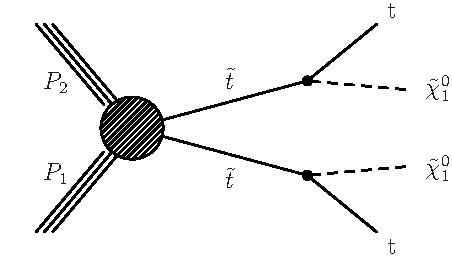
\includegraphics[width=0.50\textwidth]{sections/mc4/Introduction/figures/T2tt.pdf}\\
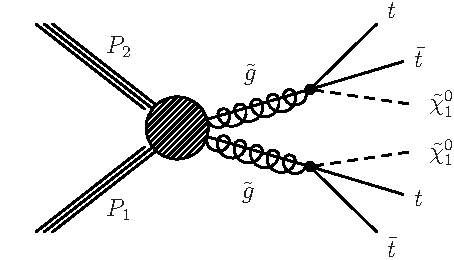
\includegraphics[width=0.40\textwidth]{sections/mc4/Introduction/figures/T1tttt_feynman.pdf}
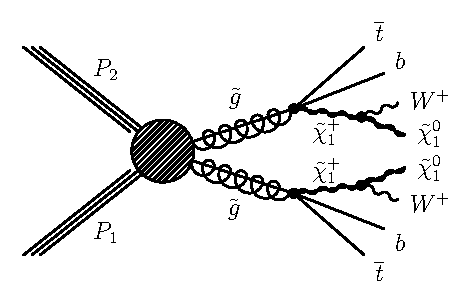
\includegraphics[width=0.40\textwidth]{sections/mc4/Introduction/figures/T1ttbb.pdf}\\
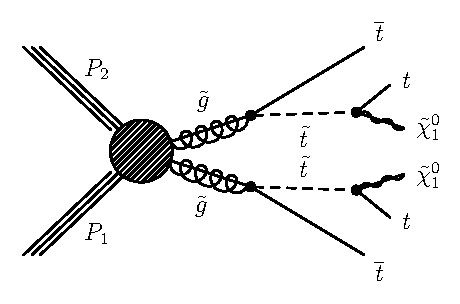
\includegraphics[width=0.40\textwidth]{sections/mc4/Introduction/figures/T5tttt.pdf}
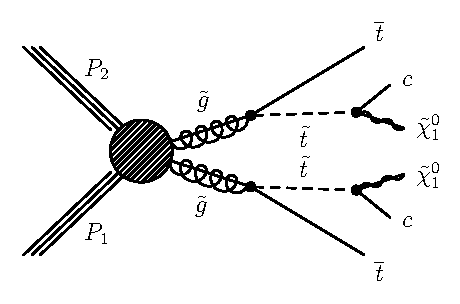
\includegraphics[width=0.40\textwidth]{sections/mc4/Introduction/figures/T5ttcc.pdf}\\
\caption{Signal models of interest in this search:
top squark pair production with the top squark decaying into a top quark and
neutralino (top),
and top squarks from cascade decays of gluinos (middle and bottom).
The SUSY simplified model topology shown at the top is referred to as T2tt,
the middle left model as T1tttt, middle right model as T1ttbb
the bottom left one as T5tttt and the bottom right one as T5ttcc.}
\label{fig:signal_diagrams}
\end{centering}
\end{figure}

The first step of the search is to design a search region with proper selection criteria. Since we are looking into all-hadronic channels, leptons and isolated tracks are vetoed. Isolated tracks are vetoed because they can arise from single-prong tau lepton decays or from electrons or muons that are not identified. Minimum requirements on the number of jets and \MET are needed to suppress the standard model background. A set of $\Delta\phi$ cuts between the \MET and several leading jets are applied to reject QCD events. Moreover, since the signal final states have tagged b-jets and top quark candidates, minimum requirements on the numbers of tagged b-jets and reconstructed top quarks are included in the baseline selection. We use the official recommendation for b tagging from the CMS b-tagging working group. However, for top quark candidates, we developed our own algorithms. For the analysis of the 2015 data, we used a cut-based top tagger approach\cite{PhysRevD.96.012004}. For the analysis of the 2016 data, described in this thesis, we designed an improved top tagger, which is described below. Several working points are designed for this top tagger.

The next step is to determine the top tagger working point and optimize the definitions of the search bins. We optimized the search bin definition for both medium and tight top tagger working points, and then chose the tight one because it is more sensitive for some signal models.

Then, we need to estimate the backgrounds for all search bins. The major background is from standard model \ttbar, $W$+jets and single top processes. The $Z$+jets, QCD, TTZ and other rare processes can be important in some search bins.

Finally, we can set limits on the model parameters by using the data yield, background estimation and expected model yields in a likelihood fit. The interpretation of data is based on simplified models\cite{Alwall:2008ag}, shown in Fig~\ref{fig:signal_diagrams}, as was already discussed.
